%!TEX TS-program = xelatex
%!TEX encoding = UTF-8 Unicode
%%========================================================
%%  编译方法(Windows, Mac OSX): 					
%%                    XeLaTeX 
%%                    biber
%%                    XeLaTeX
%%                    XeLaTeX
%%========================================================

%%%%%%%%%%%%%%%%%%%%%%%%%%%%%%%%%%%%%%%%%%%%%%%%%%%%%%%%%%
%            中文稿 文章模板:A4 纸, 五号字, 单列              
%%%%%%%%%%%%%%%%%%%%%%%%%%%%%%%%%%%%%%%%%%%%%%%%%%%%%%%%%%

\documentclass[Chinese]{APSart}
% 添加自己论文需要的其他宏包
%\usepackage{}  

\ExecuteBibliographyOptions{gblocal = gb7714-2015, 
							gbnamefmt = uppercase, 
%						    firstinits=true,
						    gbpub = false,
						    mincitenames = 1, % 要定义最后的分割符 (逗号, &, 和) , 前者:1 -> 一作等; 2-> 一作,二作 等
						    maxcitenames = 2, % 2
						    maxbibnames = 3,
						    defernumbers=true
					    }
					  
\addbibresource{apsrefs-cn.bib} % 加载bib文件(参考文献)


%%\linenumbers
\begin{document}
%\linenumbers
%\pagewiselinenumbers   

%%
%%%%%%%%%%%%%%%%%%%%%%%%%%%%%%%%%%%%%%%%%%%%%%%%%%%%%%%%%%%%%%%%
%%------------------ 编辑部提供的信息 ------------------------%%
%%%%%%%%%%%%%%%%%%%%%%%%%%%%%%%%%%%%%%%%%%%%%%%%%%%%%%%%%%%%%%%%
\newcommand{\pubvol}{XX}         % 卷号
\newcommand{\pubno}{X}           % 期号
\newcommand{\pubyear}{XXXX}      % 出版年份
\newcommand{\pubmonth}{XX}       % 出版月份
\newcommand{\enpubmonth}{xx}     % 出版月份
\newcommand{\ksym}{xx}           % 开始页码
\newcommand{\jsym}{xx}           % 结束页码
\newcommand{\receivedate}{XXXX 年 XX 月 XX 日} % 论文收到日期
\newcommand{\modifydate}{XXXX 年 XX 月 XX 日}% 论文修改日期
\newcommand{\doino}{DOI:10.3969/j.issn.1001-4268.year.month.no}
\newcommand{\citationinfo}%
{citation information, 录用后编辑部提供}
%{LIU B W, ZHANG J, CHEN X P. \etitle\,[J]. Chinese J Appl Probab Statist, \pubyear, \pubvol(\pubno): \ksym--\jsym. }
%%
\apsnumber{APS-2024-001}             % 论文编号 --- 编辑部受理后产生

%%
%%%%%%%%%%%%%%%%%%%%%%%%%%%%%%%%%%%%%%%%%%%%%%%%%%%%%%%%%%%%%%%%
%%-------------------- 作者提供的信息 ------------------------%%
%%%%%%%%%%%%%%%%%%%%%%%%%%%%%%%%%%%%%%%%%%%%%%%%%%%%%%%%%%%%%%%%
\newcommand{\runcnauthors}{作者列表}  
%作者列表格式: 一作姓名 (仅有一个作者时)
%            一作姓名, 二作姓名 (仅有二个作者时)
%            一作姓名, 等 (超过两个作者时)
\newcommand{\cnfirstauthor}{一作姓名}
\newcommand{\cnsecondauthor}{二作姓名$^\star$}
\newcommand{\cnfirstinst}{一作单位, 城市名, 邮政编码}
\newcommand{\cnsecondinst}{二作单位, 城市名, 邮政编码}
% 可添加更多作者及信息
\newcommand{\authorsinfo}{\textbf{作者信息}:~
第一作者(出生时间--),~性别,~职称,~主要研究方向:~xxxxxx,~E-mail:xxxxx@xxxx.xxx.xx~;
第二作者(出生时间--):~性别, 职称,主要研究方向:~xxxxxx,~E-mail:xxxxx@xxxx.xxx.xx~.}
\newcommand{\caemail}{abc@xyz.edu.cn}
\newcommand{\cntitle}{论文题目}
\newcommand{\hdcntitle}{页眉上论文题目}
\newcommand{\cnkeywords}{关键词1; 关键词2; 关键词3; 关键词4}
\newcommand{\cnclassno}{Oxxx.xx (网站: \url{http://www.ztflh.com/})}  % 中图分类号
\newcommand{\cnfundinfo}{XXXX基金资助~(批准号: 12345678).}
%% 中文摘要
\newcommand{\cnabstract}{摘要内容摘要内容摘要内容摘要内容摘要内容摘要内容摘要内容摘要内容摘要内容摘要内容摘要内容
	摘要内容摘要内容摘要内容摘要内容摘要内容摘要内容摘要内容摘要内容摘要内容摘要内容摘要内容摘要内容摘要内容.}
%%
%% 英文信息
\newcommand{\enfirstauthor}{First Name}
\newcommand{\ensecondauthor}{Second Name}
\newcommand{\enfirstinst}{First Author's Working Unit, City, Zip Code, Country}
\newcommand{\ensecondinst}{Second Author's Working Unit, City, Zip Code, Country}
% 可添加更多作者及信息
\newcommand{\entitle}{Article Title}
\newcommand{\hdentitle}{Article Title on page header}
\newcommand{\enkeywords}{Keyword 1; Keyword 2; Keyword 3; Keyword 4}
\newcommand{\amsno}{62xxx (网站:\url{https://mathscinet.ams.org/msc/})} % AMS Subject Claassification
\newcommand{\enfundinfo}{The project was supported by grant name(s) (Grant No(s) 1234, 5678).}
%%
%% 英文摘要
\newcommand{\enabstract}{The abstract comes here! The abstract comes here! The abstract comes here! The abstract comes here!
The abstract comes here! The abstract comes here! The abstract comes here! The abstract comes here! The abstract comes here!} %%
%%-------------------- 作者信息提供完毕 ------------------------%%
%% 论文标题页将自动生成
%% 作者转到后面的引言开始输入正文内容
%%%%%%%%%%%%%%%%%%%%%%%%%%%%%%%%%%%%%%%%%%%%%%%%%%%%%%%%%%%%%%%%
%        文章正文                                              %
%%%%%%%%%%%%%%%%%%%%%%%%%%%%%%%%%%%%%%%%%%%%%%%%%%%%%%%%%%%%%%%%
%
\title{\zihao{-2}\bf{\cntitle}
	\!\thanks{\cnfundinfo}}
\author{\zihao{-4}\kaishu{\cnfirstauthor}\\[-1pt]
	{\zihao{-5}(\cnfirstinst)}\and
	\zihao{-4}\kaishu{\cnsecondauthor}\\[-1pt]
	{\zihao{-5}(\cnsecondinst)}}
\date{} % 这一行用来去掉默认的日期显示
\maketitle
\vspace{-6mm}

%%%%%%%%%%%%%%%%%%%%%%%%%%%%%%%%%%%%%%%%%%%%%%%%%%%%%%%%%%%%%%%%
% 作者姓名与单位 : 三种形式中选一种
% 后面英文摘要中的名字和单位类似处理
% ---------------------
% 第一种形式: 仅有一个单位
% 作者列表
% (作者单位)
% ---------------------
% \author{\zihao{4}\kaishu{\cnfirstauthor}\\[-1pt]
%    {\zihao{-5}(\cnfirstinst)}}

% ---------------------
% 第二种形式: 二个单位 多个作者 --- 名字左右并列
% 作者列表1     作者列表2  
% (作者单位1)   (作者单位2)
% ---------------------
% \author{\zihao{4}\kaishu{\cnfirstauthor}\\[-1pt]
%     {\zihao{-5}(\cnfirstinst)}
%     \and 
%     {\zihao{4}\kaishu{\cnsecondauthor}}\\[-1pt]
%     {\zihao{-5}(\cnsecondinst)}}

% ---------------------
% 第三种形式: 不同单位 多个作者 -- 名字与单位上下并列
% \author{\zihao{4}\kaishu{\cnfirstauthor}\\[-1pt]
%     {\zihao{-5}(\cnfirstinst)}\\[0.8em]
% \author{\zihao{4}\kaishu{\cnsecondauthor}\\[-1pt]
%     {\zihao{-5}(\cnfirstinst)}}
%
% 其他可视为上述三种的组合
% ---------------------
%%%%%%%%%%%%%%%%%%%%%%%%%%%%%%%%%%%%%%%%%%%%%%%%%%%%%%%%%%%%%%%

%%%%%%%%%%%%%%%%%%%%%%%%%%%%%%%%%%%%%%%%%%%%%%%%%%%%%%%%%%%%%%%%
%  中文摘要
%%%%%%%%%%%%%%%%%%%%%%%%%%%%%%%%%%%%%%%%%%%%%%%%%%%%%%%%%%%%%%%%


\begin{center}
\begin{minipage}[c]{14cm}
	\zihao{-5}
	\textbf{摘~~~要:}\quad{\fangsong\cnabstract}\\
	\textbf{关键词:}\quad{\fangsong\cnkeywords}\\
	\textbf{中图分类号:}\quad\cnclassno\\
	\rule[3mm]{14cm}{0.2pt}\vskip-4mm
	\textbf{英文引用格式:} 
	\quad \fullcite{Current2024}.
	 (in Chinese)\\ %\citationinfo
		\rule[3mm]{14cm}{0.2pt}
\end{minipage}
\end{center}
\footnote[0]{\hskip-1.5mm$^\star$通讯作者, E-mail: \caemail.}
\footnote[0]{本文\receivedate{}收到, \modifydate{}收到修改稿.}\vspace{-1em}


%%%%%%%%%%%%%%%%%%%%%%%%%%%%
%  正文由此开始,请作者输入!!
%%%%%%%%%%%%%%%%%%%%%%%%%%%%
%\linenumbers
\pagewiselinenumbers   % 行号供审稿时用,投稿前可注释 


\section{导言}
这是专门为《应用概率统计》定制的中文\LaTeX{}模板, 2024年的版本5.0在2015年4.0版本的基础上作了很多的改进或优化, 定制包括页面布局、字体类型与大小、章节标题、页眉、中英文摘要、公式、图形、表格及参考文献等. 新模板具有下面的特点: 
\begin{enumerate}[leftmargin=7.8mm,itemsep=-0.1ex,label=(\arabic*)]
\item \textbf{跨平台}: 新模板可在Windows、Mac OS、Linux系统上使用,源文件使用UTF-8编码,并要求用Xe\LaTeX{}进行编译;
\item \textbf{开源免费}: 新模板秉持可持续迭代更新和兼容性,基于开源架构开发,并可在开源平台使用. 我们推荐 Windows和Linux安装并用户使用完整的TeXLive (推荐下载地址: 
\url{https://mirrors.tuna.tsinghua.edu.cn/help/CTAN/#/}), Mac OS用户安装并使用TeXLive或Mac\TeX{}; 推荐所有的用户使用TeXStudio或VS Code进行论文的排版和预览;
\item \textbf{支持Overleaf开源云平台}: 用户只要在免费共享的Overleaf平台(\url{https://www.overleaf.com/})上注册并登录帐号后就可建立一个与本模板对应的项目,接着将模板源文件(或自己正在修改中的源文件)上传到项目中就可进行论文的排版. 我们强烈推荐那些在本地电脑使用\TeX{}有问题的用户使用Overleaf. 它允许任何用户在任何时间通过任何终端(包括电脑、平板、甚至手机)的网页进行论文的排版和修改. 最新模板也将开源到Overleaf平台上, 方便更新与更多用户使用. 
\item \textbf{中英文兼容}: 新模板充分考虑到了《应用概率统计》期刊属于中英文混刊的特点,通过定制的文档类\texttt{apsart.cls}的二个选项\texttt{Chinese}和\texttt{Englsih}分别指向适用于中文与英文论文的设置文件\verb/apsart_cn.cfg/和\verb/apsart_en.cfg/来达到模板的兼容性.
\item \textbf{使用便利}: 综合考虑到录入、排版与校对的便利性,新模板对整个论文的基本信息进行了集中提取,要求作者在正式投稿前提供作者及论文的中英文信息, 见表 \ref{tab:cnart-metainfor} 和表 \ref{tab:enart-metainfor}. 在论文接受之后的排校过程中要求编辑部编辑逐步完善引用所需的bib基本信息,并生成论文DOI,详见表 \ref{tab:jeo-metainfor}. 

\begin{table}[H]
\centering\zihao{-5}
\caption{论文作者提供的中文基本信息\label{tab:cnart-metainfor}}
\begin{tabular}{lll}
\toprule
		信息         	 &  \TeX 命令              & 说明\\
\midrule
		一作等       	 & \verb/\runcnauthors/    & 作者不超过二个时全部列出,超出二个时格式为: 一作姓名, 等\\
		一作姓名(列表)   & \verb/\cnfirstauthor/   & 单名的姓与名之间加一空格, 格式为: \verb/姓\hy 名/ (其中\verb/\hy/为 10pt)\\ 
		二作姓名(列表)   & \verb/\cnsecondauthor/  & 二个作者名字之间加大空格,格式为: \verb/一作姓名\hy\hy 二作姓名/\\ 
		一作单位     	& \verb/\cnfirstinst/     & 到二级单位(院系或部门)\\ 
		二作单位     	& \verb/\cnsecondinst/    & 到二级单位(院系或部门)\\ 
		... ...     	& ... ...    			&  若有, 添加更多作者的信息\\ 
		作者信息      	& \verb/\authorsinfo/     &  编辑部存档用,包括姓名、研究方向、邮箱等\\
		通讯作者邮箱	   & \verb/\caemail/         & \\
		论文中文标题		 & \verb/\cntitle/        & \\
		论文标题缩写	   & \verb/\hdentitle/      & 在页眉中使用, 通常不必缩写\\
		论文关键词		& \verb/\cnkeywords/     & 多个关键词之间用分号分开\\
		中图分类号		& \verb/\cnclassno/      &  可从网站 \url{http://www.ztflh.com/} 获取\\
		AMS主题分类号       & \verb/\cnclassno/      & 可从网站 \url{https://mathscinet.ams.org/msc/} 获取\\
		中文基本资助信息  & \verb/\fundino/        &  多个基金用顿号和“和”分开\\
\bottomrule
\end{tabular}
\end{table}

\begin{table}[H]
\centering\zihao{-5}
\caption{论文作者需提供的英文基本信息\label{tab:enart-metainfor}}
\begin{tabular}{lll}
\toprule
		信息         &  \TeX 命令              & 说明\\
\midrule
		一作等英文   	& \verb/\runenauthors/    & 作者不超过二个时全部列出,超出二个时格式为: 一作姓名, et al.\\
		一作英文姓名     & \verb/\enfirstauthor/   & 姓在前, 且姓的字母全部大写(e.g. ZHANG J T)\\ 
		二作英文姓名     & \verb/\ensecondauthor/  & 姓在前, 且姓的字母全部大写(e.g. ZHANG J T)\\ 
		一作英文单位     & \verb/\enfirstinst/     & 到二级单位(院系或部门)\\ 
		二作英文单位     & \verb/\ensecondinst/    & 到二级单位(院系或部门)\\ 
		... ...     	& ... ...    			& 若有, 添加更多作者的信息\\ 
		论文英文标题     & \verb/\entitle/        & 除介词等小词外, 首字母大写\\
		论文英文标题简化	   & \verb/\hdentitle/ & 在页眉中使用(超出行宽时)\\
		论文英文关键词   & \verb/\enkeywords/     & 多个关键词之间用分号分开\\
		英文基金资助信息  & \verb/\enfundino/        &  多个基金用逗号和“and”分开\\
\bottomrule
\end{tabular}
\end{table}


\begin{table}[htbp]
\centering\zihao{-5}
\caption{编辑部提供的基本信息\label{tab:jeo-metainfor}}
\begin{tabular}{lll}
\toprule
信息       &  \TeX 命令      & 说明\\
\midrule
 卷号           & \verb/\pubvol/      & \\ 
 期号		   	  & \verb/\pubno/       & \\
 出版年份     	 & \verb/\pubyear/     & 示例: 2024\\
 出版月份        & \verb/\pubmonth/    & 示例: 5 \\
 出版月份        & \verb/\enpubmonth/  & 示例: May\\
 开始页码        & \verb/\ksym/        & \\
 结束页码        & \verb/\jsym/        & \\   
 论文收到日期		& \verb/\receivedate/ &  中文稿格式: XXXX 年 XX 月 XX 日\\
                &                     &  英文稿格式: Month Day, Year\\
 论文修改日期      & \verb/\modifydate/  & 中文稿格式: XXXX 年 XX 月 XX 日\\
                &                     &  英文稿格式: Month Day, Year\\
 DOI号           & \verb/\doino/        & 格式: 10.3969/j.issn.1001-4268.year.month.no\\
 引用信息         & \verb/\citationinfo/ & 与文后参考文献格式相同\\
\bottomrule
\end{tabular}
\end{table}
   
\end{enumerate}

\begin{remark}
新模板不仅给出论文录入的\TeX{}格式, 而且给出的详细的说明. 新模板受益人群包括(但不限于):
\begin{itemize}[leftmargin=7.8mm,itemsep=-0.1ex]
\item 《应用概率统计》的作者;
\item 《应用概率统计》的编校人员;
\item 负责排印的编辑. 
\end{itemize}	
\end{remark}
\begin{remark}		
假设我们的\TeX{}源文件为\texttt{myart.tex}, 则使用模板的排版流程和命令如下:
\begin{enumerate}[leftmargin=7.8mm,itemsep=-0.1ex,label=\arabic*)]
	\item Xe\LaTeX{} myart.tex
	\item bib myart.tex
	\item Xe\LaTeX{} myart.tex
	\item Xe\LaTeX{} myart.tex
\end{enumerate}
若在排版过程中没有涉及参考文献目录及引用的修改,则只须使用一次Xe\LaTeX{}进行编译. 上述命令均可在TeXstudio等平台上通过菜单或按钮运行. 
\end{remark}

为方便各类用户使用, 我们在接下来的第 \ref{floats} 节、第 \ref{bib-ref} 节和附录 \ref{remarks} 对《应用概率统计》新模板的使用作进一步的举例说明,目的是使待排论文能在极短的时间内符合期刊的基本要求,并在正式接受后可尽快达到出版的要求.  


\section{常用浮动对象的排版} \label{floats}
概率或统计类期刊论文的排版主要涉及一些浮动对象(包括章节、列表、公式、图形、表格和参考文献等带计数器的环境)的录入、编译和问题处置, 此模板对它们进行了适当的调整,这里通过一些具体的例子来说明这类浮动对象的排版、标签设定与引用. 用户可通过模板的\TeX{}源代码体会它们的具体用法. 

\subsection{章节标题}
原则上全文只列出一级标题(section)和二级标题(subsection), 三级以上标题用有序列表环境排版. 

\begin{remark}
	附录标题与正文标题不连续编号, 用附录A, 附录B等进行编号. 附录中的公式、表格和图形的编号加上附录的编号作为前缀, 详见附录 \ref{remarks}.
\end{remark}


\subsection{列表环境}
常用的列表环境分为有序列表(enumerate)和无序列表环境(itemize),新模板建议对边界和行距等用\TeX{}宏包\texttt{enumitem}对它们作适当调整. 有序列表还可用选项label对列表的编号进行修改: 
\verb/label= (\arabic*), \emph{\alph*}, (\Roman*)/, 下面是几个示例. 

\begin{enumerate}[leftmargin=7.8mm,itemsep=-0.1ex,label=\arabic*)]
	\item 有序列表1
	\item 有序列表2
	\begin{enumerate}[leftmargin=7.8mm,itemsep=-0.1ex,label=(\alph*)]
		\item 有序列表1
		\item 有序列表2
	\end{enumerate}
\end{enumerate}

\begin{enumerate}[leftmargin=7.8mm,itemsep=-0.1ex,label=(\Roman*)]
	\item 有序列表1
	\item 有序列表2
\end{enumerate}

\subsection{数学公式环境的使用}

数学公式分为行内公式(inline mode)和独立行公式(display mode), 较为复杂的数学都建议用独立行公式排版, 并在适当且必要的位置加上标签, 便于在正文中引用. 

独立行公式公式可归纳为三类, 即单行公式、分支公式和多行公式, 相应的数学类环境分别为\texttt{equation}、\texttt{cases}和\texttt{align}, 其中\texttt{cases}并不是一个纯数学环境,需要放在另一数学环境(如\texttt{equation})中. 下面给出一些示例. 
\begin{enumerate}[leftmargin=7.8mm,itemsep=-0.1ex]
\item 单行公式1: 使用\verb/\[ ... \]/, \verb/$$ ... $$/ 或  \texttt{equation*}
\[
y_1, y_2, \cdots, y_n \sim N(0,1).
\]
\item 单行公式2: 使用\texttt{equation}
\begin{equation}\label{eqn-1}
\mu(\bm x)=\beta_0 + \beta_1 x_1 + \dots + \beta_p x_p
\end{equation}	
\item 分支公式1: 使用\texttt{cases} 和 \verb/\[ ... \]/
\[ 
\sign(x)=
\begin{cases}
	-1, & \text{$x<0$}\\
	0, & \text{$x=0$}\\
	-1, & \text{$x>0$}
\end{cases} 
\]
\item 分支公式2: 使用\texttt{cases} 和 \texttt{equation}
\begin{equation}\label{eqn-2}
\sign(x)=
\begin{cases}
	-1, & \text{$x<0$}\\
	0,  & \text{$x=0$}\\
	-1, & \text{$x>0$}
\end{cases} 
\end{equation}
\item 多行公式1 (断行或各自编号): 使用\texttt{align}	
\begin{align}
	\uppi &= 3.1415926\cdots, \nonumber \\
	&\approx  3.14. \label{align-a1}\\
	\me &= 2.7182818\cdots, \label{align-a2}\\
	\upgamma &= 0.5772156\cdots .   \label{align-a3}
\end{align}
\item 多行公式2 (作为整体): 使用\texttt{aligned}和\texttt{equation}	
\begin{equation}\label{align-2}
\begin{aligned}
Y & = \beta_0 + \beta_1 X + \varepsilon, \\
\varepsilon & \sim N(0, \sigma^2). 
\end{aligned}
\end{equation}
\end{enumerate}

\begin{remark}
《应用概率统计》模板使用半角的黑点作为句点, 并要求数学公式之后加上必要的标点符号, 基本规则可归纳为: 1) 若公式是整句的结束, 则加句点; 2) 多行公式之间用逗号; 3) 公式在句子中作为主语或宾语时则不必加标点符号. 
\end{remark}	
\begin{remark}
公式环境可分为带计数器的版本与不带计数器的版本(又称为星号(*)版本),前者可通过添加标签并在正文中需要时被引用, 后者可视为前者的简化版. 
\end{remark}

\begin{remark}
多行数学公式不建议用非标准的\texttt{array}和被认为已淘汰的多行数学公式\texttt{eqnarray}环境排版.
\end{remark}

\begin{remark}
\texttt{align}有不少变形, 包括\texttt{align*}, \texttt{aligned},  \texttt{alignat}, \texttt{alignat*}, \texttt{alignedat}, \texttt{falign}等. 另外,我们还可以借助\texttt{gather}, \texttt{split}来实现超长数学公式的拆分或多行数学公式的排版. 参见文献\ncite{Gai2024,Voss2014,Gratzer2007}.  
\end{remark}

\begin{remark}
	带计数器的数学公式环境, 编号在右侧,置于圆括号中. 可用\verb|\eqref{label}|引用,其中标签\texttt{label}可通过\verb=\label{}=在被引的公式后设定. 见公式\eqref{eqn-1} 和 公式\eqref{eqn-2}. 
\end{remark}

\begin{remark}
	多行公式的编号与引用:
	\begin{itemize}[leftmargin=7.8mm,itemsep=-0.1ex]
		\item 并非所有带计数器的公式环境需要设定编号, 特别是在像\texttt{align}这样的多行数学公式环境中, 理论上系统会在每一行的数学公式后添加连续的编号, 但这通常并不是必须的. 对于不必要设定公式编号的数学公式, 其后面需要添加命令\verb/\nonumber/. 见公式\eqref{align-a1}, \eqref{align-a2}和\eqref{align-a3}.
		\item 
		对于一组多行呈现的数学公式,若这组公式之间虽然彼此相对独立但被作为一个整体来被引用,或者这组公式本身就是一个整体, 则建议给这组公式整体添加一个编号, 编号居中. 这时我们建议使用\texttt{align}的变形\texttt{aligned}加上一个\texttt{equation}环境来排版. 见公式\eqref{align-2}. 	
		\item 
		若一组多行呈现的数学公式,其前后有递进关系(例如在推导中), 则建议将公式编号设在这组公式的最后一行, 并添加标签, 因为这样的一组公式实际上是一个单一的公式,只是因排版的需要而被多次断行了. 见公式\eqref{align-a1}.	
	\end{itemize}
\end{remark}
附录 \ref{remarks} 列出了一些数学公式排版中常见的问题与处理方法. 

\subsection{三线表格环境的使用}
学术论文普遍使用三线表. 三线表的主要特点是: 整个表格通常只有三条横
线, 上下两条横线较粗, 中间一条较细. 三线表一般不使用竖线, 特别是左右两边. 结合\verb/\multicolumn/命令和\texttt{multirow}宏包中的\verb/\multirow/命令可排出非常美观的表格, 示例见表 \ref{table:1} 和表 \ref{table:2}.


\begin{table}[htbp]
\centering\zihao{-5}
\caption{用booktabs生成表格 --- 使用\texttt{multicolumn}命令. 用booktabs生成表格 --- 使用\texttt{multicolumn}命令. }\label{table:1}
\vskip -5pt
	\begin{tabular}{cccccc}
		\toprule
		& \multicolumn{4}{c}{得分} & \\
		\cmidrule(lr){2-5}
		姓名 & 数学分析 & 高等代数 & 政治 & 英语 & 总分 \\
		\midrule
		黄一天 & 90 & 85 & 92 & 88 & 355 \\
		李二虎 & 88 & 90 & 85 & 89 & 352 \\
		张三牛 & 92 & 87 & 88 & 93 & 360 \\
		\bottomrule
	\end{tabular}
\end{table}

\begin{table}[htbp]
\centering\zihao{-5}
\caption{用booktabs生成表格 --- 使用\texttt{multirow}命令.} \label{table:2}
\vskip -5pt
\begin{tabular}{ccc}
	\toprule
	Column 1 & Column 2 & Column 3\\ 
	\midrule
	\multirow{2}{*}{Multirow}&X&\multirow{2}{*}{Multirow}\\
	&X&\\
	X&\multirow{2}{*}{Multirow}&\multirow{2}{*}{Multirow}\\
	X&&\\
	\bottomrule
\end{tabular}
\end{table}
 

\subsection{图形环境的使用}
\subsubsection{单图排列}
最常用的是一个图占一行,如图 \ref{fig:1} 所示. 

\begin{figure}[htbp]
	\centering
	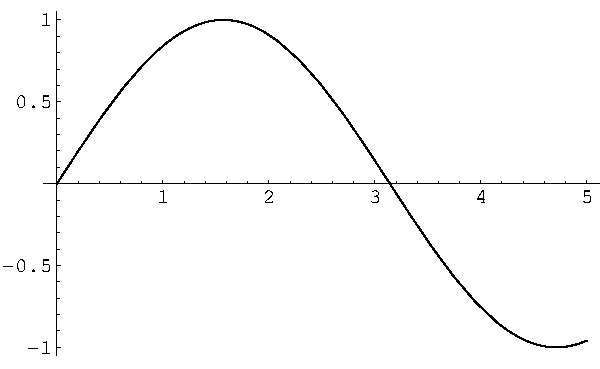
\includegraphics[width=0.55\textwidth]{figs/sin.pdf}
	\caption{单个图片\label{fig:1}}
\end{figure}


\subsubsection{图形并置 \label{chap5:figure2}}
我们常常希望将两个或多个较小的图形(称为子图)并排放在一起,传统的工具有小页环境(minipage) 和 子图环境(subfigure或subfig), 但它们都是相对较老的方法,设置较为不便. 在这个新模板中我们推荐使用新的subcaption宏包, 它不仅能完全替代前三个工具,而且提供了非常丰富的选项(可通过命令\verb/\subcaptionsetup/设置, 与caption宏包的选项相同), 用于控制或调整子图的呈现. 但要注意的是, 它与subfigure或subfig不兼容, 因此不能混合使用.  

利用subcaption宏包进行子图排版有二种方式,或是用命令\verb/\subcaptionbox/, 或是用subcaptionblock环境. 下面仅给出三个示例,  具体可参考subcaption宏包的参考手册. 

\begin{example}
两个子图并置, 且相对独立, 分别编号, 见图 \ref{mini:suba} 和 图 \ref{mini:subb}. 		
\begin{figure}[htbp] %[H]
	\centering
	\captionbox{这是第一个图. 这是第一个图. 这是第一个图. 这是第一个图.\label{mini:suba}}[0.45\textwidth]
	{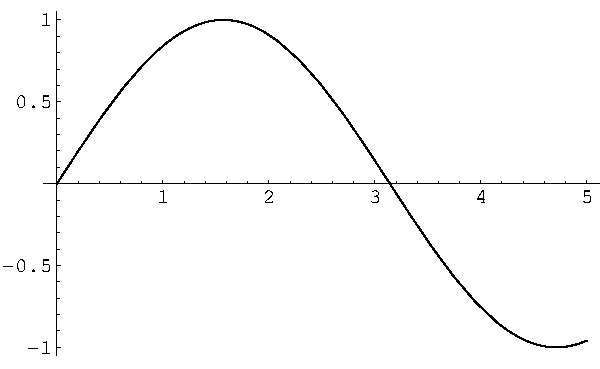
\includegraphics[width=0.4\textwidth]{figs/sin.pdf}}
	%\hfil
	\captionbox{这是第二个图. 这是第二个图. 这是第二个图. 这是第二个图.\label{mini:subb}}[0.45\textwidth]
	{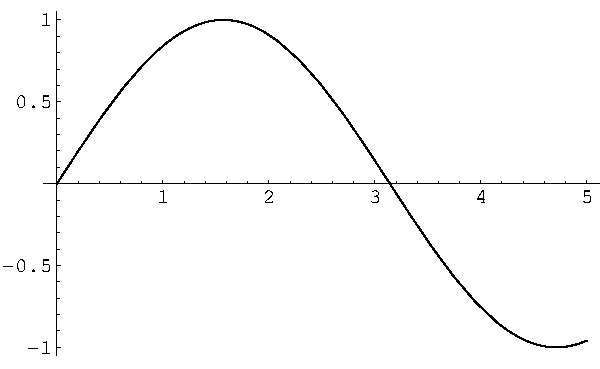
\includegraphics[width=0.4\textwidth]{figs/sin.pdf}}
	%	\caption{二个图形并置}
	%	\label{mini:subfigs} %% label for entire figure
\end{figure}
\end{example}

\begin{example}
用命令\verb/\subcaptionbox/实现两个子图并置, 且形成整体, 带一个主编号和两个子编号, 见图 \ref{mini:subfigs}. 	

\begin{figure}[htbp] %[H]
	\centering
	\subcaptionbox{这是第一个图. 这是第一个图. 这是第一个图. 这是第一个图\label{mini:subc}}[0.45\textwidth]
		{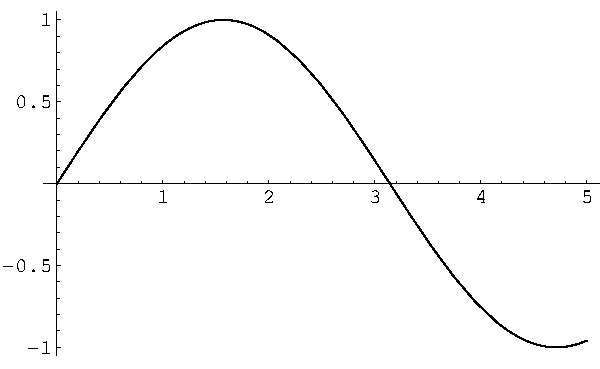
\includegraphics[width=0.4\textwidth]{figs/sin.pdf}}
	%\hfil
	\subcaptionbox{这是第二个图. 这是第二个图. 这是第二个图. 这是第二个图. \label{mini:subd}}[0.45\textwidth]
		{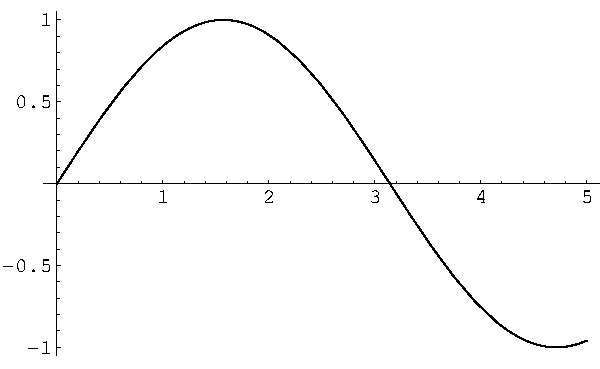
\includegraphics[width=0.4\textwidth]{figs/sin.pdf}}
	\caption{二个图形并置(使用subcaptionbox命令). 二个图形并置(使用subcaptionbox命令). 二个图形并置(使用subcaptionbox命令). }
	\label{mini:subfigs} %% label for entire figure
\end{figure}

\end{example}

\begin{example}
用环境\verb/\subcaptionblock/实现两个子图并置, 且形成整体, 带一个主编号和两个子编号. 见图 \ref{mini:subfigures} . 		
\begin{figure}[H]
	\centering
	\begin{subcaptionblock}{0.45\textwidth}	
		\centering
		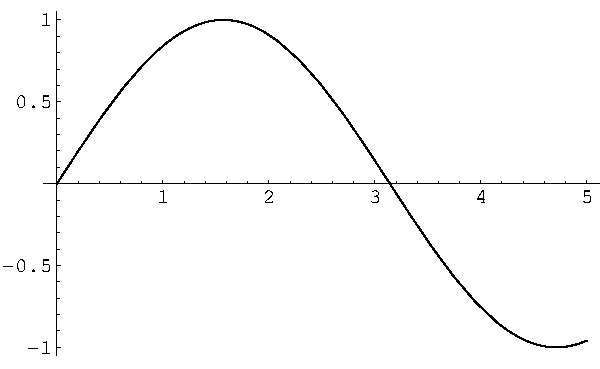
\includegraphics[width=0.8\textwidth]{figs/sin.pdf}
		\caption{这是第一个图}\label{mini:sube} 
	\end{subcaptionblock}%	
	%\hfil
	\begin{subcaptionblock}{0.45\textwidth}	
		\centering
		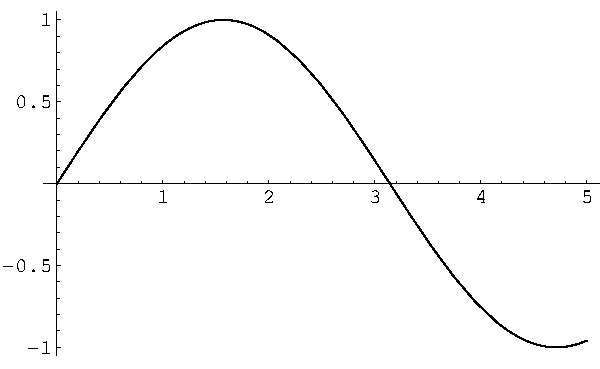
\includegraphics[width=0.8\textwidth]{figs/sin.pdf}
		\caption{这是第二个图}\label{mini:subf} 
	\end{subcaptionblock}	
	\caption{二个图形并置(使用subcaptionblock环境)}\label{mini:subfigures} 
\end{figure}
\end{example}

\begin{remark}
表格(table)和图形(figure)的编号居中,都使用\verb|\ref{label}|引用, 其中标签\texttt{lable}可通过\verb=\lable{}=设定.
\end{remark}
\subsection{定理类环境定制}
定理类环境包括定理(theorem)、引理(lemma)、推论(corollary)、命题(proposition)、性质(property)、假设(assumption)、例子(example)、问题(question)、记号(notation)、注释(remark)等, 编号在左侧, 也用\verb|\ref{lable}|和\verb|\lable{}|引用和设定标签. 《应用概率统计》要求定理、引理、推论、命题和性质共享一个计数器,即它们连续编号,而其余定义的环境独立编号. 
下面给出一些示例.  
\begin{definition} %
	这是定义内容.
\end{definition}%
\begin{lemma}%
	这是引理内容.
\end{lemma}
\begin{theorem}\label{thm-1}%
	这是定理\ref{thm-1}内容.
\end{theorem}%
\begin{proof}%
	这是定理的证明.
\end{proof}
\begin{theorem}\label{thm-2}{[唯一性定理]}\;
	这是定理 \ref{thm-2} 的内容.
\end{theorem}%
\begin{corollary}%
	这是推论.
\end{corollary}
\begin{proposition}
	这是一个命题的内容.
\end{proposition}
\subsection{浮动对象的引用}
下面是一些引用的例子:
\begin{example}
	这里引用了第\pageref{align-2}页的公式 \eqref{align-2}.
\end{example}
\begin{example}
	这里引用了第 \pageref{table:1} 页的表 \ref{table:1}.
\end{example}
\begin{example}
	这里引用了第 \pageref{mini:subd} 页的图 \ref{mini:subf}.
\end{example}
\begin{example}
	这里引用了第 \pageref{thm-1} 页的定理 \ref{thm-1}.
\end{example}


\section{参考文献录入、生成与引用}\label{bib-ref}
参考文献是一类特殊的浮动对象, 在此进行单独说明. 
新的模板采用bib建立文献数据库,并采用由胡振震定制的符合国家标准GB/T7714-2015 的 biblatex 参考文献样式管理参考文献的生成与引用,

示例\texttt{apsref-cn.bib}中罗列了常用的文献类型与相应的条目, 例如一篇典型的期刊论文的bib条目如下:
\begin{verbatim}
	@Article{biblabel, 
		title   = {标题}, 
		author  = {作者, 多个作者用 and 连接}, 
		journal = {期刊名}, 
		volume  = {卷20}, 
		number  = {页码}, 
		pages   = {开始页码 -- 终止页码}, 
		year    = {年份}, 
	}
\end{verbatim} 
其中\texttt{biblabel}是为此文献取的标签,建议采用第一作者的姓加发表年份的组合,便于引用且保证全文基本重复, 例如\texttt{Fisher:1957}, . 

\begin{remark}
本模板采用传统的数字编号方式, 参考文献编号在左侧,置于方括号中, 本模板根据\texttt{bilatex}宏包设定了四种引用方式:
\begin{enumerate}[leftmargin=7.8mm,itemsep=-0.1ex,label= \arabic*)]%\emph{\alph*},(\Roman*),(\arabic*)
	\item 一般引用, 使用\verb|\ncite{}|, 例如: 见文献\ncite{Dengjs01};
	\item 带附加信息引用, 使用自定义命令\verb|\rcite{}|引用, 如文献\rcite{Gelman2014}{第186页}, 文献\rcite{Gelman2014}{第三章第2节定理2};
	\item 上标形式引用, 使用自定义命令\verb|\ucite{}|,例如: 进一步的学习相关的参考文献\ucite{Wuwei:2013,Lip04,Sangdy01,Dengjs01,Chenzj02}; 
	\item 带作者姓的引用, 使用\verb|\ancite{}|, 例如 \ancite{Wuwei:2013}(仅有一个作者), \ancite{Sangdy01}(仅有二个作者),  以及\ancite{Dengjs01}(三个以上作者) 给出了大量实际的案例供我们学习使用. 
\end{enumerate}
\end{remark}	

\begin{remark}
有三个及以上作者的文献目录仅列出三个,引用时仅列出一个, 例如: \ancite{Mao2003}, \ancite{Gelman2014}. 	
\end{remark}

\begin{remark}
由于本模板是基于biblatex实现文献库的管理, 文献目录按引用顺序依次列出, 因此作者一旦修改了参考文献,或者在正文中的引用顺序发生了变化,必须用\texttt{biber}引擎对库进行更新,这样再次编译时会自动更新文献目录和引用的编号.	\texttt{biber}引擎的用法与与bibtex类似, 但更为灵活.
\end{remark}



%%%%%%%%%%%%%%%%%%%%%%%%%%%%%%%%%%%%%%%%%%%%%%%%%%%%%%%%%%%%%%%%
%        文章附录                                               %
%%%%%%%%%%%%%%%%%%%%%%%%%%%%%%%%%%%%%%%%%%%%%%%%%%%%%%%%%%%%%%%%
%
\appendix
\numberwithin{equation}{section}
\numberwithin{figure}{section}
\numberwithin{table}{section}
\makeatletter 
% "activate" the preparatory code, but for section-level headers only
\newcommand{\section@cntformat}{附录 \thesection:\ }
\makeatother

%%%%%%%%%%%%%%%%%%%%%%%%%%%%%%%%%%%%%%%%%%%%%%%%%%%%%%%%%%%%%%%%
\section{特别说明}\label{remarks}
%%%%%%%%%%%%%%%%%%%%%%%%%%%%%%%%%%%%%%%%%%%%%%%%%%%%%%%%%%%%%%%%

新模板对数学符号、函数或表达式根据现有的期刊规范和年审要求重新进行了处理.
\begin{enumerate}[leftmargin=7.8mm,itemsep=-0.1ex, label=(\arabic*)]
\item 数学花体: 使用命令\verb/\mathscr{}/或缩略形式\verb|\scr{}|及重新定义的\verb|\cal{}|命令, 例如 \verb/$\mathscr{A}, \scr{B}, \cal{C}$/ 分别产生 $\mathscr{A}, \scr{B}, \cal{C}$;
\item 数学粗体: 由于
\verb|\mathbb{}|命令对数字失效,一种解决方案是使用宏包mathbbold,但考虑到在Mac OSX的Mac\TeX{}上宏包mathbbold没有安装, 此模板对此命令进行了重新定义. 例如, 
\verb/$\mathbb{A,B,R}, \mathbold{1}$/产生$\mathbb{A,B,R}, \mathbbold{1}$.
\item 数学黑体:有二种解决方案,一是直接使用\texttt{bm}宏包中的命令\verb|\bm|, 其二是使用本模板定义的\verb|\bm| 命令\verb/\newcommand{\bm}{\boldsymbol}/, 它对 
数字、英文字母和希腊字母均有效, 例如,
\verb|\bm{2\ Greeks $\alpha$, $\Gamma$}|产生 $\bm{2\ Greeks}$ $\bm{\alpha}$, $\bm{\Gamma}$.
\item 省略号: 尽管\verb|\dots|能智能识别省略号的位置,但它并不符合国家标准中的相关规定,在年检时可能会导致扣分或警告. 为些,我们要求作者将所有的省略号用居中的格式排版,即用\verb/\cdots/来排版. 例如,  
由\verb=$1+2+ \dots + n$= 得到 $1+2+ \dots + n$, 这是正确的. 但用
\verb/$i=1, 2, \dots, k$/ 却得到 $i=1, 2, \dots, k$. 按年检要求应改为\verb/$i=1, 2, \cdots, k$/,  得到 $i=1, 2, \cdots, k$.
\item 数学函数: \TeX{}使用\verb|\func(x)|, 例如 \verb|\log(y)|,\verb|\exp(z)|, \verb|\max| 分别产生
$\sin(x)$, $\log(y)$, $\exp(z)$, $\max$. 表 \ref{fig:mathfuns} 列出了\TeX{}系统相关数学宏包中常用的函数. 但概率统计类的论文经常会遇到一些\TeX{}系统没有定义的函数,需要我们自己定义, 表 \ref{tab:mathfuns} 列出了此模板常用的一些自定义函数. 

\begin{figure}[htbp]
	\centering
	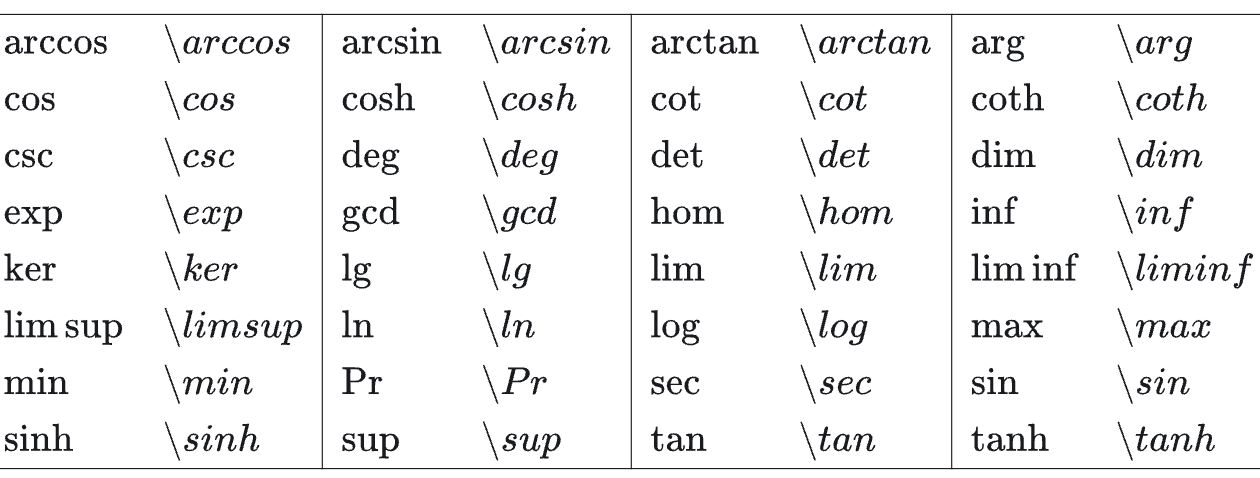
\includegraphics[width=0.85\textwidth]{figs/texmathop.png}
	\caption{\TeX{}系统定义的数学函数\label{fig:mathfuns}}
\end{figure}

\begin{table}[H]
\centering\zihao{-5}
\caption{自定义数学函数/算子\label{tab:mathfuns}}
\begin{tabular}{lll}
\toprule
函数名       &  \TeX 命令      & 示例\\
\midrule
数学期望     & \verb/\ep/      & $\ep(X)$\\
方差        & \verb/\var/    & $\var(X),\sin(X)$\\
协方差(阵)   & \verb/\cov/    & $\cov(X)$\\
概率         & \verb/\pr/     & $\pr(X>0)$ (cf. $\Pr(X>0)$)\\
标准差      & \verb/\std/    & $\std(X)$\\
相关系数(阵)  & \verb/\cor/    & $\cor(X)$\\
矩阵求迹      & \verb/\tr/    & $\tr(X)$\\
矩阵拉直      & \verb/\vect/    & $\vect(X)$\\
符号函数     & \verb/\sign/     & $\sign(\delta)$\\
微分         & \verb/\md/     & $\md x$\\
\bottomrule
\end{tabular}
\end{table}
\item 数学公式中的常数: $\me$、$\uppi$(圆周率)和$\upgamma$(欧拉常数)不能视为符号用数学符号用斜体$e$、$\pi$和$\gamma$, 除非它们确实代表的是参数或变量. 例如, 比较下面二种标准正态分布的密度函数排版的差异,
\[
\phi(x)=\frac{1}{\sqrt{2\uppi}\sigma^2} \me^{-\frac{(x-\mu)^2}{2\sigma^2}}\hy \text{(正确)}; \qq
\phi(x)=\frac{1}{\sqrt{2\pi}\sigma^2} e^{-\frac{(x-\mu)^2}{2\sigma^2}}\hy \text{(错误)}.
\]
\item 向量与矩阵的转置: \TeX{}有专门的转置符 $\top$, 而不用字母\texttt{T}. 例如
\[
\bm{\hat\beta}=(\bm X^\top \bm X)^{-1}\bm X^\top \bm Y.
\] 
\item 带帽类符号的大小的调整: 对于小写的英语字母和希腊字母用\verb/\hat/, \verb/\tilde/, \verb/\bar/, 而对于对于大写的英语字母、大写的希腊字母和更宽的组合符号用\verb/\widehat/, \verb/\widetilde/, \verb/\widebar/更合适或美观, 其中\verb/\widebar/是模板中自定义的, 它比\verb/\overline/ 及\texttt{mathabx}中的相应命令更显美观些. 下面是一个示例. 
\begin{equation}\label{eqn-5}
\widehat{\Theta}=\sum_{z} \frac{n(\boldsymbol{z})}{n}\left\{\widebar{Y}_{a}(\boldsymbol{z})
	-\widetilde{Y}_{b}(\boldsymbol{z})\right\}. 
\end{equation}
\item 定界符: 定界符是成对出现的, 主要有\verb/( )/, \verb/[ ]/, \verb/{ }/, \verb/< >/, \verb/| |/. 我们应尽可能使用\verb/\left ... \right/让系统自动匹配定界符的高度. 对于仅在单侧出现的定界符, 为了让其保持公式相当的高度, 在另一侧用\verb/\left./ 或 \verb/\right./ 与之进行匹配. 在此仅举二个特殊的例子, 其中公式\eqref{eqn-6}是通过单侧定界符及在定界符之间使用\verb/\middle|/来解决的. 
\begin{equation}\label{eqn-6}
\left.\frac{1+\bigl\{\,x\times[\,f(x)+g(x)\,]\,\bigr\}}{\sqrt{a+b}} \right|_{x=0} 
=\left.\left(\,\frac{c}{a+b}\,\right)^{1/2}\middle/ \left(\,\frac{\ln c}{\ln a+ \ln b}\,\right)^{1/2}\right..
\end{equation}
而下面的公式\eqref{eqn-7}还涉及定界符不允许分割的问题. 
\begin{align}
	P&\left(n_{1}\left(M_{1, n_{1}}-1\right) \leq n_{1}\left(\frac{x}{a_{2, n_{2}}}+b_{2, n_{2}}-1\right),\right.\nonumber\\
	&\quad\left. \vphantom{\left(\frac{x}{a_{2, n_{2}}}+b_{2, n_{2}}-1\right)}
	a_{2, n_{2}}\left(M_{2, n_{2}}-b_{2, n_{2}}\right) \leq x\right) .\label{eqn-7}
\end{align}
此例中使用了 \verb/\vphantom{expr}/ 用于读取一个与 \texttt{expr} 表达式相同高度的空盒子,并置于第二行的(单侧)定界符 \verb/\left. .../\  \verb/\right)/ 中, 这样让它与第一行的(单侧)定界符 \verb/\left( ... \right./ 组合在一起得到一个左右高度完全一样的完美的定界符对\verb/\left( ... \right)/. 
\end{enumerate}




\nocite{*}

%\setlength{\bibitemsep}{10pt}
%\addtolength{\itemsep}{-0.8 em} % 缩小参考文献间的垂直间距


\begin{spacing}{1.0} % 行距
	\printbibliography[keyword={cn},resetnumbers=true,
	                   title={\bfseries\sffamily \zihao{-4}参考文献}]
\end{spacing}	

\nolinenumbers
%%%%%%%%%%%%%%%%%%%%%%%%%%%%%%%%%%%%%%%%%%%%%%%%%%%%%%%%%%%%%%%%
%  英文摘要
%%%%%%%%%%%%%%%%%%%%%%%%%%%%%%%%%%%%%%%%%%%%%%%%%%%%%%%%%%%%%%%%
\vspace{6mm}\hspace{-8mm}
\parbox{\textwidth}{
\begin{center}
	\zihao{4}{\bf{\entitle}}\\[1em]
	\textrm{\zihao{5}\enfirstauthor}\\[0.2em]
	(\zihao{-5}\enfirstinst)\\[0.8em]
	\textrm{\zihao{5}\ensecondauthor}\\[0.2em]
	(\zihao{-5}\ensecondinst)
\end{center}
\zihao{-5}
\textbf{Abstract:}\quad\enabstract\\
\textbf{Keywords:}\quad\enkeywords\\
\textbf{2020 Mathematics Subject Classification:}\quad\amsno}
%
% 作者及单位信息不同格式参考英文论文的模板
% 

%%%%%%%%%%%%%%%%%%%%%%%%%%%%%%%%%%%%%%%%%%%%%%%%%%%%%%%%%%%%%%%%
%  文章结束
%%%%%%%%%%%%%%%%%%%%%%%%%%%%%%%%%%%%%%%%%%%%%%%%%%%%%%%%%%%%%%%%
\clearpage
\end{document}
